\documentclass{amsart}
\usepackage{graphicx}
\graphicspath{{./}}
\usepackage{hyperref}
\usepackage{csvsimple}
\usepackage{longtable}
\usepackage{lscape}
\usepackage{epigraph}
\title{Ve Ask Ze Kweszions Here: Zulf Wants to Know What is the Full Spectrum Possible for Discrete Random Variables} 
\author{Zulfikar Moinuddin Ahmed}
\date{\today}
\begin{document}
\maketitle

\section{Unsatisfactory State of Binomial and Poisson}

The Universe is a Four-Sphere governed by S4 Electromagnetic Law.  The matter and other electrically charged particle distribution in the universe is completely beyond all bounds of comprehension.  You will tell me, with a straight face, that in this complicated situation that, "Don't worry but Binomial and Poisson is all she wrote.  Take a Binomial and Poisson pill and every discrete data will seem Binomial and Poisson."  Are you totally insane?  Do you think Zulf is a fool?  Who do you think you are?  You think you're Bill Gates?  You're going to fool Zulf and the world for five decades?  No no no.  Zulf is not compelled at all.

\section{Classification Problems in Mathematics}

When I started Princeton in 1991, I was enamoured of topology and geometry, and thought I would spend my life on those sorts of problems.  In mathematics, the classification of two-dimensional compact manifolds by topology occurred late nineteenth to early twentieth century.  Henri Poincare began the process formalising topology -- 'analysis situs' he called it -- and then after tremendous amount of work, Grigory Perelman completed the program of three-dimensional manifolds and their classification by proving the Poincare Conjecture early in the twenty first century.  These are some of the great highlights of mathematical achievements.  Mathematicians have classified finite simple groups as well.  Therefore I want to consider whether discrete stochastic phenomena in the entire actual universe could be put into a classificatory scheme of any validity.  I won't work on this problem for all my life, but I would like to formulate the problem and consider whether it is a problem of substance.  I am extremely dissatisfied with what there exists regarding discrete random phenomena today, mostly because I dislike games of chance and hate it when games of chance are brought into the Sacred Ruminations on Nature to which I am naturally devoted.

\section{Zulf's Principle of Noise Distributions in Nature}

I believe strongly that all Noise Distributions in this universe are {\em push-forwards of the uniform measures on the two-sphere or four-sphere by some reasonable set of maps}.  These maps are
\[
\zeta: S^2 \rightarrow \mathbf{C}
\]
In particular I showed recently that the generalised hyperbolic distribution arises in this way.  This is important because I needed to assure myself that actual noise distributions do have concentration in closed bounded intervals of $\mathbf{R}$ without which Science would be impossible in this universe because we could not get any approximation to true value of any measured variables by methods that are sensible.

\section{Vast Possibilities for Discrete distributions}

Consider any $g \in L^2(\mathbf{R})$.  Now for any $q \in \mathbf{Z}$ define $g_q = \int_{q}^{q+1} |g(x)|^2 dx$.  Voila, we have a distribution on $\mathbf{Z}$.  We can now have a count measure based on $g$, probability of $q$ things is $g_q$.  

This is so broad that the possibilities for measures on count data is infinite dimensional.  That's just obvious real analysis.  

Why is statistics going to tell us something absurd, that Binomial and Poisson are the only distributions that matter?  That is so outrageous that I have no words for it.

\section{Regardless of All Other Contingencies Statisticians Will be Blamed if Science Goes of the Rails and Falls off Grand Canyon}

Statisticians can be proud of their work for good reasons.  And still Scientists will be lazy and just apply some statistical procedure and publish reams of papers in all the top journals without worry.  They will say, "such and such statistician says so."  To them, statisticians are telling them, "Use my procedure and ye shall know the Truth of Nature and the Truth shall set you free."  Then when all of Science is a heap of rubbish at the bottom of Grand Canyon because the Scientists trusted the Statisticians, who will they blame?  Not themselves, be assured.  They will execute the whole cadre of Statisticians and try to save their own skins when the public is outraged that they paid huge amount of taxes and the Scientists got everything wrong and all the children went insane waiting for the summer rain and so on.

\section{Total Irrelevance of Ethnicity the Moment Real Threats to Lives and Reputations of Scientists Arise}

People like Bill Gates are idiots because they think Ethnicity matters.  In any Apocalyptic scenario, no one will give a crap about Ethnicity.  Scientists of all Ethnicities will tribe themselves under severe public pressures everywhere in the world and blame Statisticians of all Ethnicities for all sorts of problems.  {\em That} is human nature too, and that human nature is also shared across all Ethnicities.  I have never encountered any man or woman of any ethnicity who will not blame everyone else if there is a giant problem and billions of people are ready to hang them.  They won't give a crap about ethnicity.  They'll say, "We did what we thought was right.  We relied on those guys over there, you see those arrogant Statisticians of all Ethnicities who think they know more than Muhammad and Jesus Christ?  Blame them, not us."

\section{Statisticians Have Serious Responsibilities}

Statisticians are not dilettantes.  Now I am a devotee of Nature, not a Statistician, but a devotee of Nature.  I consider Nature's Laws to be Sacred, and I sing hymns; I sit and stare at the Sun seeking greater insights into the heart of Nature.  I am obsessed with beautiful situation where the most fleeting of all, we, human beings, who are not comfortable in our interpreted world can see beyond seeing itself and contemplate the what was not our creation, life, existence and so on.  I don't have time to do all the work of Statisticians for them.  They are obligated to give me tools that work, procedures that do not distract Zulf from focus on contemplation of all things of Heaven and Earth.  I want statistical procedures that make my life easier, where I can quickly pronounce great advances of Man's Understanding of deeper reality and so on.  Do you have any idea how enraged I get when I have spent months examining the true beauty of all sorts of things of unearthly beauty and the goddam statistical procedures don't want to give me the sort of confidence I want to share with people, especially the lovely ladies?  

It is intolerable when Statistics does not deliver.  Who cares what fine tuned consideration you have for all sorts of Bayesian Markov Chain Monte Carlo procedures if your procedures do not allow Zulf to see beyond seeing itself?

\section{Frequentist and Bayesian Inference Theories Are Insufficient}

A theory of statistical inference in the void is meaningless.  The real issue is how someone devoted to the truth of Nature, the true laws of Nature, is able to be confident that what he or she has found is actually the true laws of Nature.  That is the enterprise of Science.  We rely on Statistics to tell us how to do this.  We have our theories, the various schemes of mere Man, and we have overweening ambitions, to secure from Nature her most intimate secrets.  We rely on Statisticians to provide us with the means to be confident that what we do leads to either confidence that these are truly the laws of Nature or to tell us that Nature is displeased and will not share her secrets.  We cannot tolerate these sorts of Inference theories that are unreliable.  Neither Frequentist nor Bayesian hypotheses are relevant to this great task.  You have to do better than this.  This is just nonsense!  What do you mean Frequentist claptrap?  Do you really think Nature will abide by these horribly primitive hypotheses?  And what does nature care about Subjective Probabilities of all sorts of egomaniacs?  Nature {\em does not care about these thing!}

\section{Large Class of Poisson Measures}

For any measure $\nu$ on $\mathbf{R}$ and any $\alpha>0$ define
\begin{equation}
\pi_{\nu,\alpha} = e^{\alpha}\sum_{n=0}^\infty \frac{\alpha^n}{n!} \nu^{*n}
\end{equation}
This is developed in Dan Stroock's {\em Probability Theory an Analytic Theory} book.  

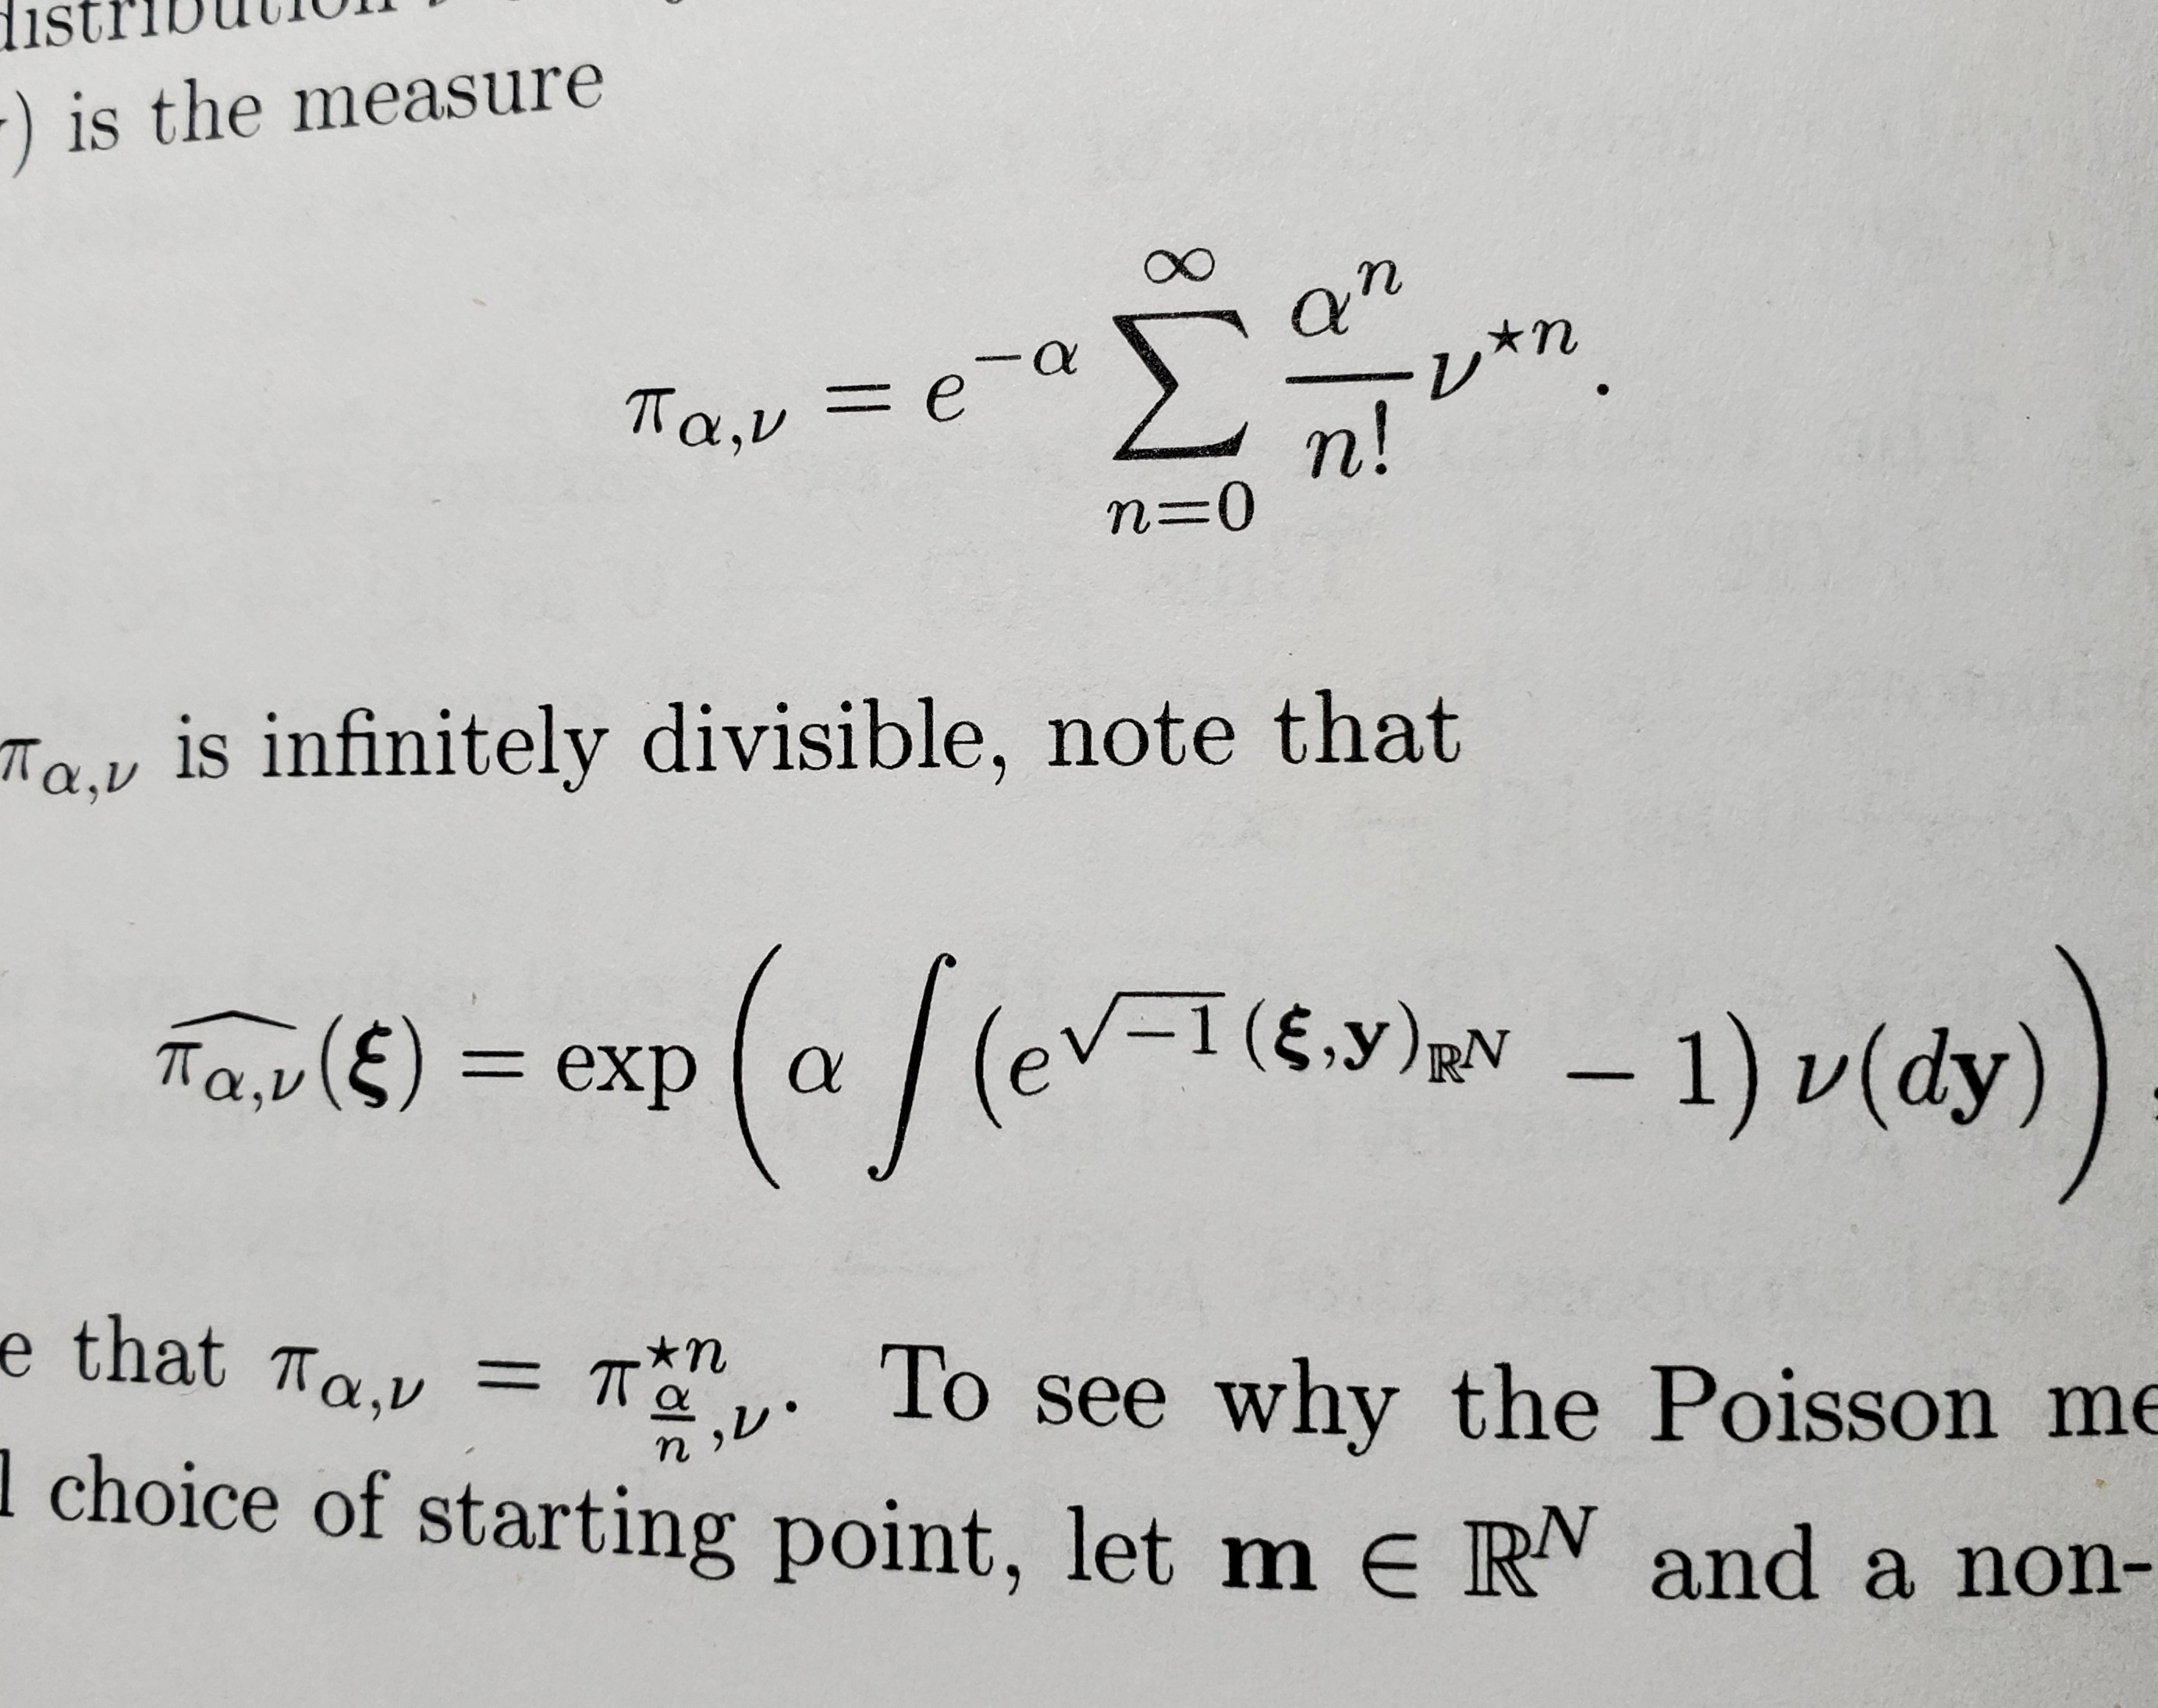
\includegraphics[rotate=270,scale=0.1]{danbook.jpg}

I worked with Dan 1999-2000 and he's a very talented mathematician.  Everyone should read his beautiful book.

Pick any $g\in\ell^2(\mathbf{Z})$ and define
\[
\nu = \sum_{r = \infty}^\infty \delta_r \int_{r}^{r+1} |g|^2 dx
\]
And now we have a large class of measures that charge only integers and are all infinitely divisible. In order to see why, note that the Fourier series for these are all exponentials of the Fourier transform of $\nu$ and therefore positive.  These are a large infinitely divisible family of probability distributions on $\mathbf{Z}$.  One suspects that a large subclass of these could be quite valuable in models of count data that are much better models than taking Poisson distributions and tweaking it to increase dispersion in ad hoc manner which is the bread and butter of count data analysis today.

Now why would Statistics not tell us which of these are valuable for Nature models and which of them are not valuable?  

\section{Legacy of Simeon-Denis Poisson}

I am not an erudite historian of Mathematics and Statistics, but I have very good scientific sense.  Simeon-Denis Poisson in 1837 proved that as probability of success goes to zero, binomial approaches Poisson distribution.  He was also quite active in Poisson summation and other formulae with Fourier series.  But at the time of course infinite divisibility was not a concept; this was introduced by de Finetti in 1920s and masterfully studied by Paul Levy.  Reversing history, we can see that the tools needed to have a deeper understanding of infinitely divisible distributions on $\mathbf{Z}$ was available to Poisson, and that is the key insight I can see, that spectral analysis is the only way to understand what is unique about probability distributions on $\mathbf{Z}$ with vast families of infinitely divisible laws.  This is bound to change the future of Science.

Now I am focused on distributions on finite sets, so I won't go too far in this direction but count data is ubiquitous, and so this is a vast area to understand in the future.

\end{document}